\documentclass[border=4pt]{standalone}
\usepackage{amsmath,amssymb}
\usepackage{tikz}
\usetikzlibrary{arrows.meta}
\begin{document}
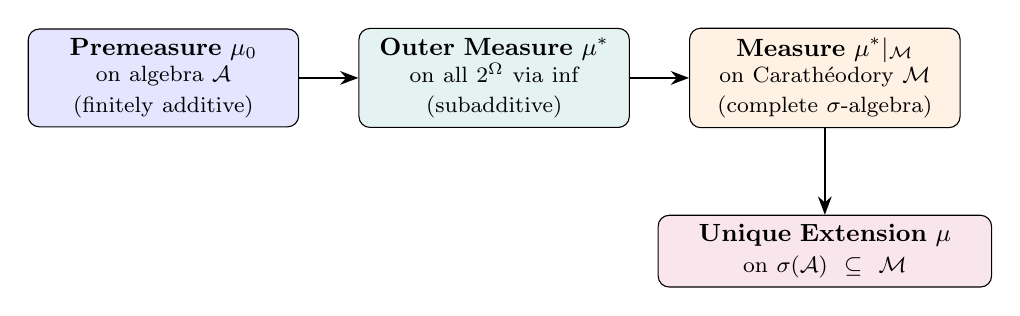
\begin{tikzpicture}[font=\small, >=Stealth]
  \node[draw, rounded corners, fill=blue!10, text width=3.2cm, align=center] (A) at (0,0)
    {\textbf{Premeasure} $\mu_0$ \\ \footnotesize on algebra $\mathcal{A}$ \\ (finitely additive)};
  \node[draw, rounded corners, fill=teal!10, text width=3.2cm, align=center] (B) at (4.2,0)
    {\textbf{Outer Measure} $\mu^*$ \\ \footnotesize on all $2^\Omega$ via inf \\ (subadditive)};
  \node[draw, rounded corners, fill=orange!10, text width=3.2cm, align=center] (C) at (8.4,0)
    {\textbf{Measure} $\mu^*|_\mathcal{M}$ \\ \footnotesize on Carathéodory $\mathcal{M}$ \\ (complete $\sigma$-algebra)};
  \node[draw, rounded corners, fill=purple!10, text width=4.0cm, align=center] (D) at (8.4,-2.2)
    {\textbf{Unique Extension} $\mu$ \\ \footnotesize on $\sigma(\mathcal{A}) \subseteq \mathcal{M}$};

  \draw[->, thick] (A) -- (B);
  \draw[->, thick] (B) -- (C);
  \draw[->, thick] (C) -- (D);
\end{tikzpicture}
\end{document}